
%(BEGIN_QUESTION)
% Copyright 2006, Tony R. Kuphaldt, released under the Creative Commons Attribution License (v 1.0)
% This means you may do almost anything with this work of mine, so long as you give me proper credit

An orifice plate is used to measure the flow rate of diesel fuel exiting the processing unit at an oil refinery where the customary unit for liquid flow measurement within refineries is ``barrels per hour'' (bbl/hr).  Calculate the following parameters in this flow measurement loop, at two different flow rates (10 bbl/hr and 31 bbl/hr):

$$\includegraphics[width=15.5cm]{i00725x01.eps}$$

\begin{itemize}
\item {} {\bf At a flow rate of 10 bbl/hr:}
\vskip 5pt
\item{} Orifice plate $\Delta$P = \underbar{\hskip 50pt} " H$_{2}$O
\vskip 5pt
\item{} Differential pressure transmitter output signal = \underbar{\hskip 50pt} PSI
\vskip 5pt
\item{} Square root extractor output signal = \underbar{\hskip 50pt} PSI
\vskip 5pt
\item{} Flow indicator reading = \underbar{\hskip 50pt} bbl/hr
\end{itemize}

\vskip 10pt

\begin{itemize}
\item {} {\bf At a flow rate of 31 bbl/hr:}
\vskip 5pt
\item{} Orifice plate $\Delta$P = \underbar{\hskip 50pt} " H$_{2}$O
\vskip 5pt
\item{} Differential pressure transmitter output signal = \underbar{\hskip 50pt} PSI
\vskip 5pt
\item{} Square root extractor output signal = \underbar{\hskip 50pt} PSI
\vskip 5pt
\item{} Flow indicator reading = \underbar{\hskip 50pt} bbl/hr
\end{itemize}

\underbar{file i00725}
%(END_QUESTION)





%(BEGIN_ANSWER)

\noindent
{\bf Partial answer:}

\begin{itemize}
\item {} {\bf At a flow rate of 10 bbl/hr:}
%\vskip 5pt
%\item{} Orifice plate $\Delta$P = \underbar{\bf 9.375} " H$_{2}$O
\vskip 5pt
\item{} Differential pressure transmitter output signal = \underbar{\bf 3.75} PSI
\vskip 5pt
\item{} Square root extractor output signal = \underbar{\bf 6} PSI
%\vskip 5pt
%\item{} Flow indicator reading = \underbar{\bf 10} bbl/hr
\end{itemize}

\vskip 10pt

\begin{itemize}
\item {} {\bf At a flow rate of 31 bbl/hr:}
\vskip 5pt
\item{} Orifice plate $\Delta$P = \underbar{\bf 90.09} " H$_{2}$O
%\vskip 5pt
%\item{} Differential pressure transmitter output signal = \underbar{\bf 10.21} PSI
%\vskip 5pt
%\item{} Square root extractor output signal = \underbar{\bf 12.3} PSI
\vskip 5pt
\item{} Flow indicator reading = \underbar{\bf 31} bbl/hr
\end{itemize}

%(END_ANSWER)





%(BEGIN_NOTES)

$$Q = k \sqrt{\Delta P}$$

At a volumetric flow rate of 40 barrels per hour and a corresponding differential pressure of 150 "WC, the value of $k$ will be 3.266.

\begin{itemize}
\item {} {\bf At a flow rate of 10 bbl/hr:}
\vskip 5pt
\item{} Orifice plate $\Delta$P = \underbar{\bf 9.375} " H$_{2}$O
\vskip 5pt
\item{} Differential pressure transmitter output signal = \underbar{\bf 3.75} PSI
\vskip 5pt
\item{} Square root extractor output signal = \underbar{\bf 6} PSI
\vskip 5pt
\item{} Flow indicator reading = \underbar{\bf 10} bbl/hr
\end{itemize}

\vskip 10pt

\begin{itemize}
\item {} {\bf At a flow rate of 31 bbl/hr:}
\vskip 5pt
\item{} Orifice plate $\Delta$P = \underbar{\bf 90.09} " H$_{2}$O
\vskip 5pt
\item{} Differential pressure transmitter output signal = \underbar{\bf 10.21} PSI
\vskip 5pt
\item{} Square root extractor output signal = \underbar{\bf 12.3} PSI
\vskip 5pt
\item{} Flow indicator reading = \underbar{\bf 31} bbl/hr
\end{itemize}

\vfil \eject

\noindent
{\bf Prep Quiz:}

If the volumetric flow rate through an orifice plate suddenly doubles, the differential pressure it produces will:

\begin{itemize}
\item{} Halve (${1 \over 2} \times$) 
\vskip 5pt 
\item{} Remain the same
\vskip 5pt 
\item{} Double (2$\times$)
\vskip 5pt 
\item{} Triple (3$\times$)
\vskip 5pt 
\item{} Quadruple (4$\times$)
\vskip 5pt 
\item{} Increase by 8$\times$ 
\end{itemize}



%INDEX% Measurement, flow: orifice plate loop calculations

%(END_NOTES)


